
\documentclass[8pt]{article}
%	options include 12pt or 11pt or 10pt
%	classes include article, report, book, letter, thesis

\usepackage[a4paper,bindingoffset=0.2in,%
            left=0.6in,right=0.6in,top=0.2in,bottom=0.4in,%
            footskip=.15in]{geometry}
            
\usepackage[T1]{fontenc}
\usepackage[polish]{babel}
\usepackage[utf8]{inputenc}
\usepackage{lmodern}
\selectlanguage{polish}
\usepackage{blindtext}
\usepackage{pgfplots}
\usepackage{graphicx}


\title{Aplikacje uniwersalne}
\author{Projekt / Semestr 6\\ Aleksander Kosma\\grupa 2 tester-programista}
\date{20 Marzec 2018}

\begin{document}
\maketitle 

\section*{Dokumentacja projektu}
\subsection*{ Opis projektu - Gym Progress}
Aplikacja ma pomóc w notowaniu progresu z siłowni. Można aplikacje wykorzystać wszędzie tam gdzie mamy kontakt z zapisem ćwiczeń w formie seria-powtórzenie. Dzięki zebranym danym aplikacja będzie mogła podać statystyki i metadane odnośnie naszych zmagań.
\subsection*{ Opis przypadków użycia}
Spis najważniejszych funkcjonalności aplikacji:\\
\textbf{Dodaj trening} - w tej aktywności użytkownik odnotowuje ćwiczenia które wykonał na treningu. Z listy wybiera konkretne ćwiczenie, następnie ustala ilość serii i ciężar.\\

\textbf{Dodaj ćwiczenie} - użytkownik może dodać nowe ćwiczenie jeśli nie ma go jeszcze na liście dostępnych.\\

\textbf{Wyświetl progres} - Aplikacja sumuje ciężar z każdego treningu i zamieszcza dane w formie tabeli. Możliwe będą różne opcje wyświetlania danych.\\

\textbf{Wyświetl treningi} - korzystający będzie mógł przeglądać dodane wcześniej treningi jak i je edytować lub usuwać.

\subsection*{ Koncept wyglądu aplikacji}
Poniżej znajduję się prawdopodobny wygląd menu aplikacji:
\begin{center}
 \makebox[\textwidth]{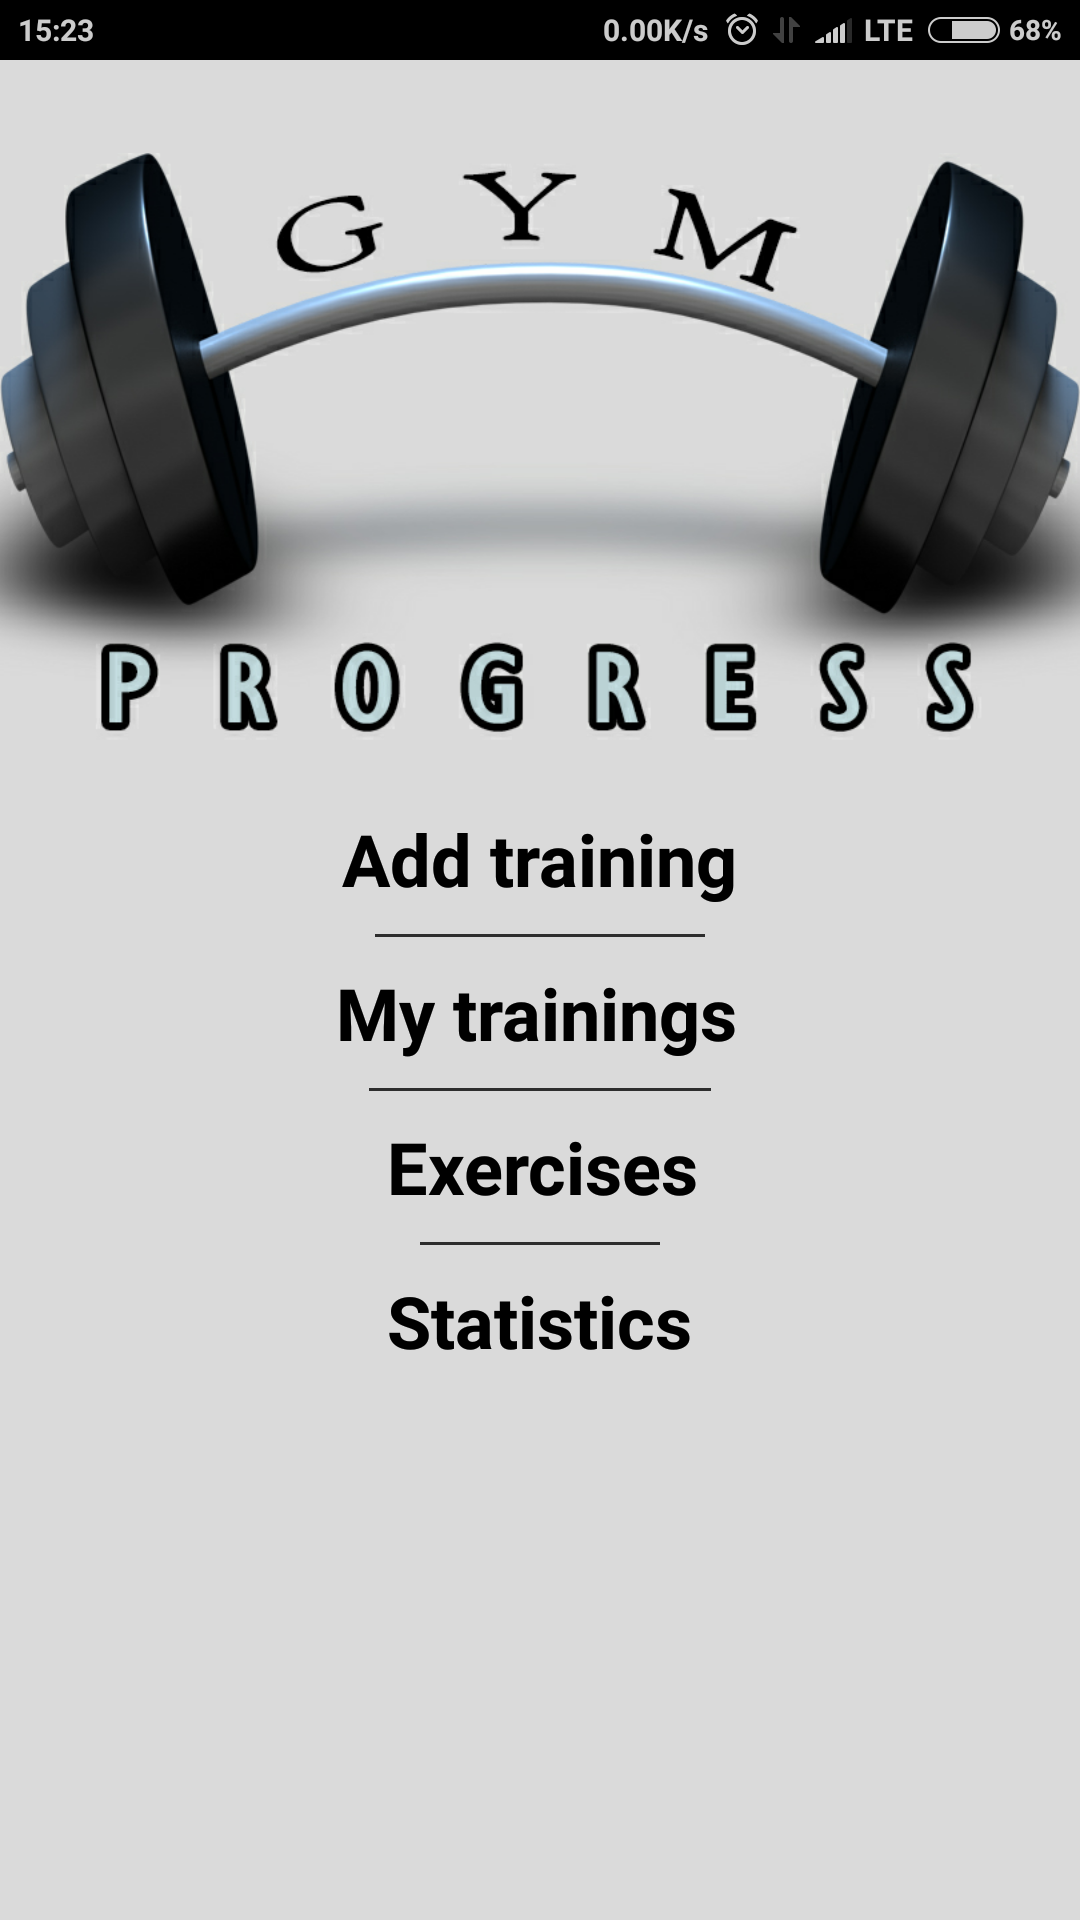
\includegraphics[width=6.75cm,height=12cm]{menu.png}}
\end{center}






\end{document}